\documentclass[1p]{elsarticle_modified}
%\bibliographystyle{elsarticle-num}

%\usepackage[colorlinks]{hyperref}
%\usepackage{abbrmath_seonhwa} %\Abb, \Ascr, \Acal ,\Abf, \Afrak
\usepackage{amsfonts}
\usepackage{amssymb}
\usepackage{amsmath}
\usepackage{amsthm}
\usepackage{scalefnt}
\usepackage{amsbsy}
\usepackage{kotex}
\usepackage{caption}
\usepackage{subfig}
\usepackage{color}
\usepackage{graphicx}
\usepackage{xcolor} %% white, black, red, green, blue, cyan, magenta, yellow
\usepackage{float}
\usepackage{setspace}
\usepackage{hyperref}

\usepackage{tikz}
\usetikzlibrary{arrows}

\usepackage{multirow}
\usepackage{array} % fixed length table
\usepackage{hhline}

%%%%%%%%%%%%%%%%%%%%%
\makeatletter
\renewcommand*\env@matrix[1][\arraystretch]{%
	\edef\arraystretch{#1}%
	\hskip -\arraycolsep
	\let\@ifnextchar\new@ifnextchar
	\array{*\c@MaxMatrixCols c}}
\makeatother %https://tex.stackexchange.com/questions/14071/how-can-i-increase-the-line-spacing-in-a-matrix
%%%%%%%%%%%%%%%

\usepackage[normalem]{ulem}

\newcommand{\msout}[1]{\ifmmode\text{\sout{\ensuremath{#1}}}\else\sout{#1}\fi}
%SOURCE: \msout is \stkout macro in https://tex.stackexchange.com/questions/20609/strikeout-in-math-mode

\newcommand{\cancel}[1]{
	\ifmmode
	{\color{red}\msout{#1}}
	\else
	{\color{red}\sout{#1}}
	\fi
}

\newcommand{\add}[1]{
	{\color{blue}\uwave{#1}}
}

\newcommand{\replace}[2]{
	\ifmmode
	{\color{red}\msout{#1}}{\color{blue}\uwave{#2}}
	\else
	{\color{red}\sout{#1}}{\color{blue}\uwave{#2}}
	\fi
}

\newcommand{\Sol}{\mathcal{S}} %segment
\newcommand{\D}{D} %diagram
\newcommand{\A}{\mathcal{A}} %arc


%%%%%%%%%%%%%%%%%%%%%%%%%%%%%5 test

\def\sl{\operatorname{\textup{SL}}(2,\Cbb)}
\def\psl{\operatorname{\textup{PSL}}(2,\Cbb)}
\def\quan{\mkern 1mu \triangleright \mkern 1mu}

\theoremstyle{definition}
\newtheorem{thm}{Theorem}[section]
\newtheorem{prop}[thm]{Proposition}
\newtheorem{lem}[thm]{Lemma}
\newtheorem{ques}[thm]{Question}
\newtheorem{cor}[thm]{Corollary}
\newtheorem{defn}[thm]{Definition}
\newtheorem{exam}[thm]{Example}
\newtheorem{rmk}[thm]{Remark}
\newtheorem{alg}[thm]{Algorithm}

\newcommand{\I}{\sqrt{-1}}
\begin{document}

%\begin{frontmatter}
%
%\title{Boundary parabolic representations of knots up to 8 crossings}
%
%%% Group authors per affiliation:
%\author{Yunhi Cho} 
%\address{Department of Mathematics, University of Seoul, Seoul, Korea}
%\ead{yhcho@uos.ac.kr}
%
%
%\author{Seonhwa Kim} %\fnref{s_kim}}
%\address{Center for Geometry and Physics, Institute for Basic Science, Pohang, 37673, Korea}
%\ead{ryeona17@ibs.re.kr}
%
%\author{Hyuk Kim}
%\address{Department of Mathematical Sciences, Seoul National University, Seoul 08826, Korea}
%\ead{hyukkim@snu.ac.kr}
%
%\author{Seokbeom Yoon}
%\address{Department of Mathematical Sciences, Seoul National University, Seoul, 08826,  Korea}
%\ead{sbyoon15@snu.ac.kr}
%
%\begin{abstract}
%We find all boundary parabolic representation of knots up to 8 crossings.
%
%\end{abstract}
%\begin{keyword}
%    \MSC[2010] 57M25 
%\end{keyword}
%
%\end{frontmatter}

%\linenumbers
%\tableofcontents
%
\newcommand\colored[1]{\textcolor{white}{\rule[-0.35ex]{0.8em}{1.4ex}}\kern-0.8em\color{red} #1}%
%\newcommand\colored[1]{\textcolor{white}{ #1}\kern-2.17ex	\textcolor{white}{ #1}\kern-1.81ex	\textcolor{white}{ #1}\kern-2.15ex\color{red}#1	}

{\Large $\underline{12a_{1001}~(K12a_{1001})}$}

\setlength{\tabcolsep}{10pt}
\renewcommand{\arraystretch}{1.6}
\vspace{1cm}\begin{tabular}{m{100pt}>{\centering\arraybackslash}m{274pt}}
\multirow{5}{120pt}{
	\centering
	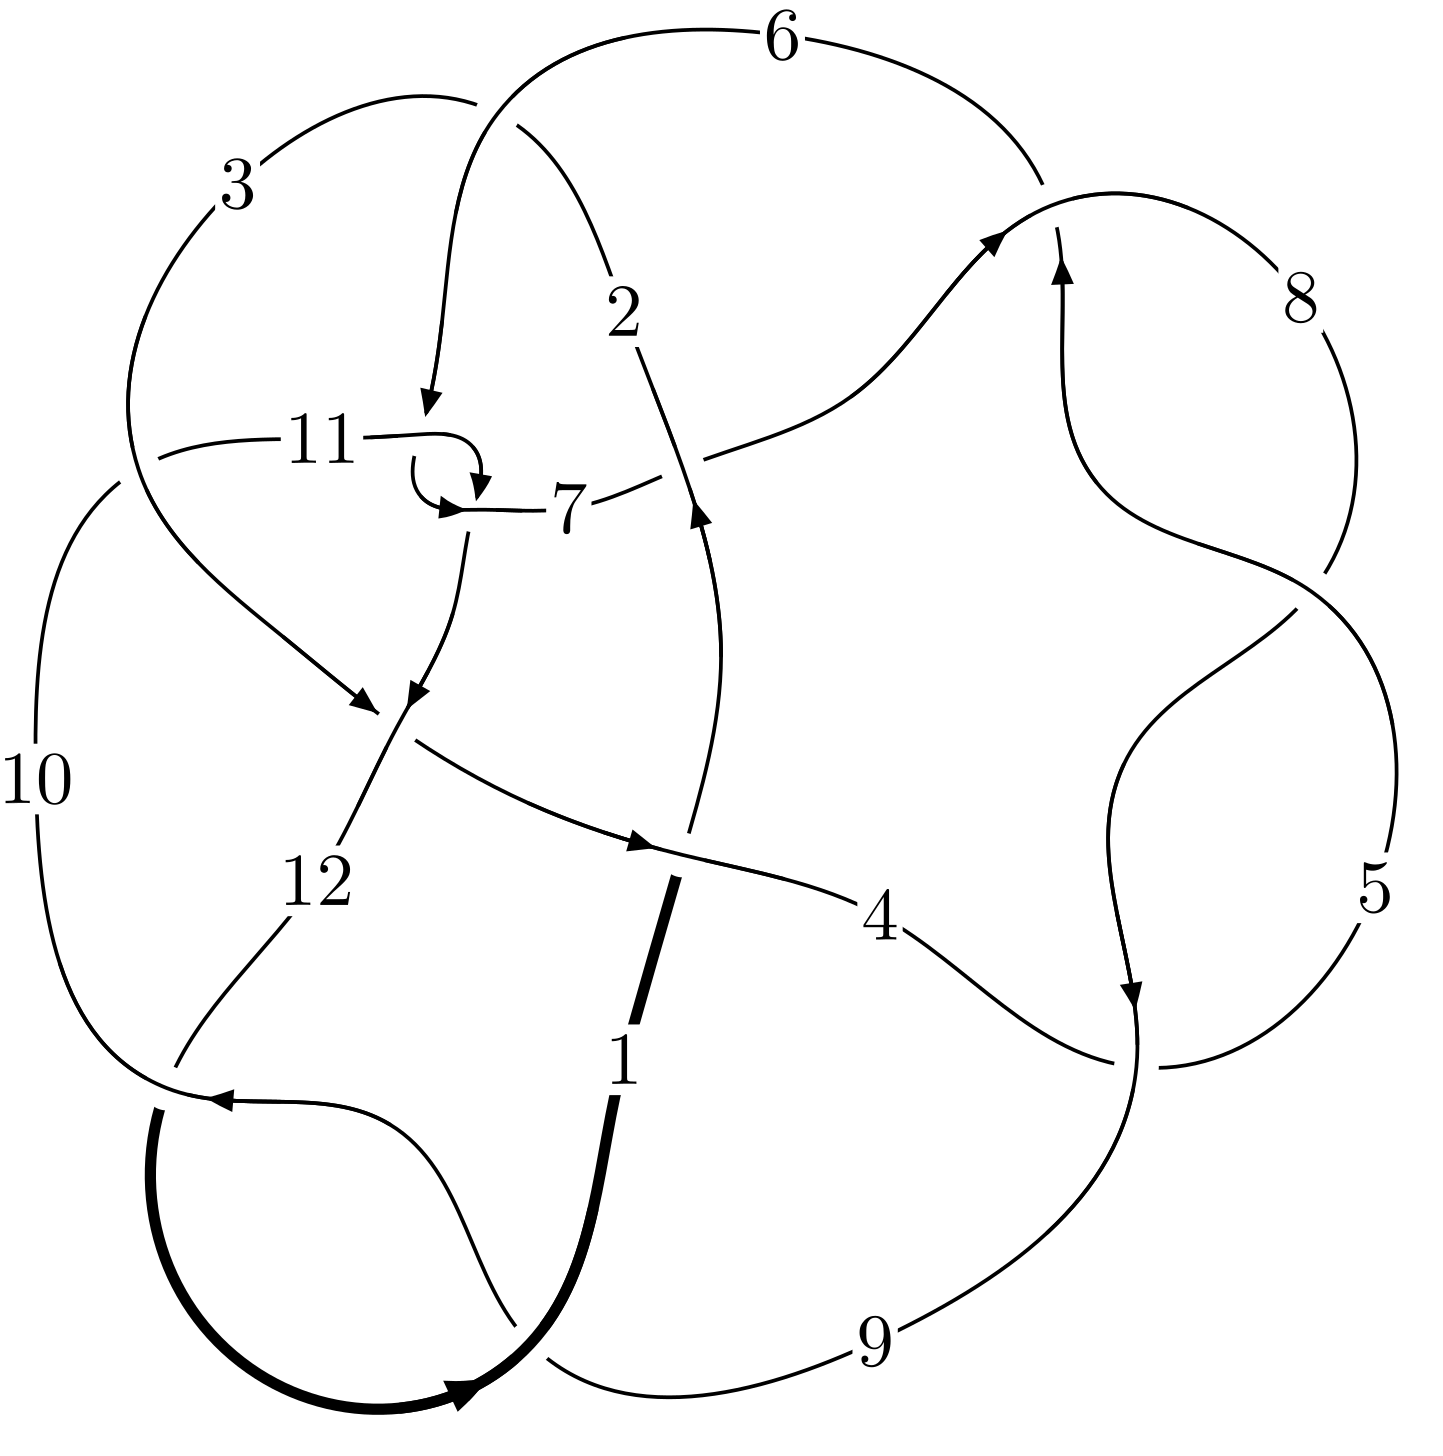
\includegraphics[width=112pt]{../../../GIT/diagram.site/Diagrams/png/1802_12a_1001.png}\\
\ \ \ A knot diagram\footnotemark}&
\allowdisplaybreaks
\textbf{Linearized knot diagam} \\
\cline{2-2}
 &
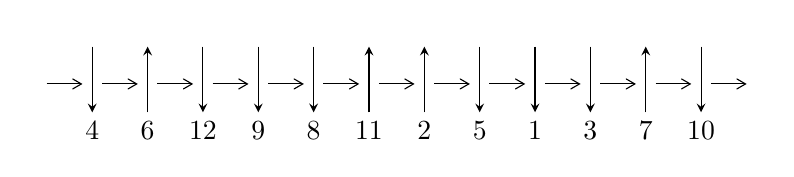
\begin{tikzpicture}[x=20pt, y=17pt]
	% nodes
	\node (C0) at (0, 0) {};
	\node (C1) at (1, 0) {};
	\node (C1U) at (1, +1) {};
	\node (C1D) at (1, -1) {4};

	\node (C2) at (2, 0) {};
	\node (C2U) at (2, +1) {};
	\node (C2D) at (2, -1) {6};

	\node (C3) at (3, 0) {};
	\node (C3U) at (3, +1) {};
	\node (C3D) at (3, -1) {12};

	\node (C4) at (4, 0) {};
	\node (C4U) at (4, +1) {};
	\node (C4D) at (4, -1) {9};

	\node (C5) at (5, 0) {};
	\node (C5U) at (5, +1) {};
	\node (C5D) at (5, -1) {8};

	\node (C6) at (6, 0) {};
	\node (C6U) at (6, +1) {};
	\node (C6D) at (6, -1) {11};

	\node (C7) at (7, 0) {};
	\node (C7U) at (7, +1) {};
	\node (C7D) at (7, -1) {2};

	\node (C8) at (8, 0) {};
	\node (C8U) at (8, +1) {};
	\node (C8D) at (8, -1) {5};

	\node (C9) at (9, 0) {};
	\node (C9U) at (9, +1) {};
	\node (C9D) at (9, -1) {1};

	\node (C10) at (10, 0) {};
	\node (C10U) at (10, +1) {};
	\node (C10D) at (10, -1) {3};

	\node (C11) at (11, 0) {};
	\node (C11U) at (11, +1) {};
	\node (C11D) at (11, -1) {7};

	\node (C12) at (12, 0) {};
	\node (C12U) at (12, +1) {};
	\node (C12D) at (12, -1) {10};
	\node (C13) at (13, 0) {};

	% arrows
	\draw[->,>={angle 60}]
	(C0) edge (C1) (C1) edge (C2) (C2) edge (C3) (C3) edge (C4) (C4) edge (C5) (C5) edge (C6) (C6) edge (C7) (C7) edge (C8) (C8) edge (C9) (C9) edge (C10) (C10) edge (C11) (C11) edge (C12) (C12) edge (C13) ;	\draw[->,>=stealth]
	(C1U) edge (C1D) (C2D) edge (C2U) (C3U) edge (C3D) (C4U) edge (C4D) (C5U) edge (C5D) (C6D) edge (C6U) (C7D) edge (C7U) (C8U) edge (C8D) (C9U) edge (C9D) (C10U) edge (C10D) (C11D) edge (C11U) (C12U) edge (C12D) ;
	\end{tikzpicture} \\
\hhline{~~} \\& 
\textbf{Solving Sequence} \\ \cline{2-2} 
 &
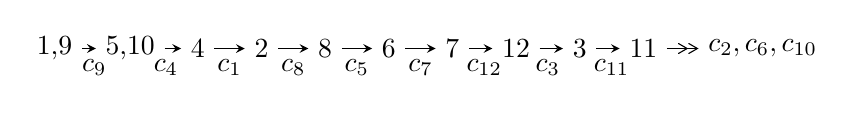
\begin{tikzpicture}[x=23pt, y=7pt]
	% node
	\node (A0) at (-1/8, 0) {1,9};
	\node (A1) at (17/16, 0) {5,10};
	\node (A2) at (17/8, 0) {4};
	\node (A3) at (25/8, 0) {2};
	\node (A4) at (33/8, 0) {8};
	\node (A5) at (41/8, 0) {6};
	\node (A6) at (49/8, 0) {7};
	\node (A7) at (57/8, 0) {12};
	\node (A8) at (65/8, 0) {3};
	\node (A9) at (73/8, 0) {11};
	\node (C1) at (1/2, -1) {$c_{9}$};
	\node (C2) at (13/8, -1) {$c_{4}$};
	\node (C3) at (21/8, -1) {$c_{1}$};
	\node (C4) at (29/8, -1) {$c_{8}$};
	\node (C5) at (37/8, -1) {$c_{5}$};
	\node (C6) at (45/8, -1) {$c_{7}$};
	\node (C7) at (53/8, -1) {$c_{12}$};
	\node (C8) at (61/8, -1) {$c_{3}$};
	\node (C9) at (69/8, -1) {$c_{11}$};
	\node (A10) at (11, 0) {$c_{2},c_{6},c_{10}$};

	% edge
	\draw[->,>=stealth]	
	(A0) edge (A1) (A1) edge (A2) (A2) edge (A3) (A3) edge (A4) (A4) edge (A5) (A5) edge (A6) (A6) edge (A7) (A7) edge (A8) (A8) edge (A9) ;
	\draw[->>,>={angle 60}]	
	(A9) edge (A10);
\end{tikzpicture} \\ 

\end{tabular} \\

\footnotetext{
The image of knot diagram is generated by the software ``\textbf{Draw programme}" developed by Andrew Bartholomew(\url{http://www.layer8.co.uk/maths/draw/index.htm\#Running-draw}), where we modified some parts for our purpose(\url{https://github.com/CATsTAILs/LinksPainter}).
}\phantom \\ \newline 
\centering \textbf{Ideals for irreducible components\footnotemark of $X_{\text{par}}$} 
 
\begin{align*}
I^u_{1}&=\langle 
3.93846\times10^{410} u^{123}+2.26334\times10^{411} u^{122}+\cdots+1.71029\times10^{411} b-2.33575\times10^{412},\\
\phantom{I^u_{1}}&\phantom{= \langle  }-8.53978\times10^{410} u^{123}-6.18776\times10^{411} u^{122}+\cdots+1.71029\times10^{411} a+3.24698\times10^{412},\\
\phantom{I^u_{1}}&\phantom{= \langle  }u^{124}+8 u^{123}+\cdots+560 u+32\rangle \\
I^u_{2}&=\langle 
-318371092 u^{29}+1036982687 u^{28}+\cdots+1519247218 b+8755986098,\\
\phantom{I^u_{2}}&\phantom{= \langle  }84610383 u^{29}+282766245 u^{28}+\cdots+3038494436 a+19372377016,\;u^{30}- u^{29}+\cdots-32 u+4\rangle \\
\\
\end{align*}
\raggedright * 2 irreducible components of $\dim_{\mathbb{C}}=0$, with total 154 representations.\\
\footnotetext{All coefficients of polynomials are rational numbers. But the coefficients are sometimes approximated in decimal forms when there is not enough margin.}
\newpage
\renewcommand{\arraystretch}{1}
\centering \section*{I. $I^u_{1}= \langle 3.94\times10^{410} u^{123}+2.26\times10^{411} u^{122}+\cdots+1.71\times10^{411} b-2.34\times10^{412},\;-8.54\times10^{410} u^{123}-6.19\times10^{411} u^{122}+\cdots+1.71\times10^{411} a+3.25\times10^{412},\;u^{124}+8 u^{123}+\cdots+560 u+32 \rangle$}
\flushleft \textbf{(i) Arc colorings}\\
\begin{tabular}{m{7pt} m{180pt} m{7pt} m{180pt} }
\flushright $a_{1}=$&$\begin{pmatrix}0\\u\end{pmatrix}$ \\
\flushright $a_{9}=$&$\begin{pmatrix}1\\0\end{pmatrix}$ \\
\flushright $a_{5}=$&$\begin{pmatrix}0.499318 u^{123}+3.61796 u^{122}+\cdots-301.498 u-18.9850\\-0.230280 u^{123}-1.32337 u^{122}+\cdots+223.187 u+13.6570\end{pmatrix}$ \\
\flushright $a_{10}=$&$\begin{pmatrix}1\\u^2\end{pmatrix}$ \\
\flushright $a_{4}=$&$\begin{pmatrix}0.269037 u^{123}+2.29459 u^{122}+\cdots-78.3102 u-5.32792\\-0.230280 u^{123}-1.32337 u^{122}+\cdots+223.187 u+13.6570\end{pmatrix}$ \\
\flushright $a_{2}=$&$\begin{pmatrix}-0.189282 u^{123}-1.38263 u^{122}+\cdots+102.831 u+2.53366\\0.0856813 u^{123}+0.393010 u^{122}+\cdots-147.048 u-8.35132\end{pmatrix}$ \\
\flushright $a_{8}=$&$\begin{pmatrix}-0.0202511 u^{123}-0.458635 u^{122}+\cdots-40.4152 u-12.0426\\0.281230 u^{123}+2.63215 u^{122}+\cdots+157.158 u+11.1424\end{pmatrix}$ \\
\flushright $a_{6}=$&$\begin{pmatrix}-0.812210 u^{123}-5.85729 u^{122}+\cdots+433.653 u+22.6467\\0.570616 u^{123}+3.66425 u^{122}+\cdots-379.706 u-22.6495\end{pmatrix}$ \\
\flushright $a_{7}=$&$\begin{pmatrix}0.188853 u^{123}+0.923993 u^{122}+\cdots-231.382 u-20.5808\\0.152414 u^{123}+1.85479 u^{122}+\cdots+257.304 u+16.3548\end{pmatrix}$ \\
\flushright $a_{12}=$&$\begin{pmatrix}u\\u^3+u\end{pmatrix}$ \\
\flushright $a_{3}=$&$\begin{pmatrix}0.289775 u^{123}+1.56030 u^{122}+\cdots-388.413 u-23.1243\\-0.113816 u^{123}+0.173382 u^{122}+\cdots+416.531 u+24.6669\end{pmatrix}$ \\
\flushright $a_{11}=$&$\begin{pmatrix}-0.363981 u^{123}-2.94441 u^{122}+\cdots-106.608 u+3.55885\\0.452720 u^{123}+3.74556 u^{122}+\cdots+87.4958 u+2.58917\end{pmatrix}$\\&\end{tabular}
\flushleft \textbf{(ii) Obstruction class $= -1$}\\~\\
\flushleft \textbf{(iii) Cusp Shapes $= -0.865722 u^{123}-7.01651 u^{122}+\cdots+103.882 u+11.6286$}\\~\\
\newpage\renewcommand{\arraystretch}{1}
\flushleft \textbf{(iv) u-Polynomials at the component}\newline \\
\begin{tabular}{m{50pt}|m{274pt}}
Crossings & \hspace{64pt}u-Polynomials at each crossing \\
\hline $$\begin{aligned}c_{1}\end{aligned}$$&$\begin{aligned}
&u^{124}+30 u^{122}+\cdots+85438383 u+36885536
\end{aligned}$\\
\hline $$\begin{aligned}c_{2}\end{aligned}$$&$\begin{aligned}
&u^{124}-29 u^{122}+\cdots-23801512 u+5726284
\end{aligned}$\\
\hline $$\begin{aligned}c_{3}\end{aligned}$$&$\begin{aligned}
&u^{124}+4 u^{122}+\cdots-31546 u+3791
\end{aligned}$\\
\hline $$\begin{aligned}c_{4},c_{5},c_{8}\end{aligned}$$&$\begin{aligned}
&u^{124}-4 u^{123}+\cdots-975 u+79
\end{aligned}$\\
\hline $$\begin{aligned}c_{6},c_{11}\end{aligned}$$&$\begin{aligned}
&u^{124}+2 u^{123}+\cdots+597 u+931
\end{aligned}$\\
\hline $$\begin{aligned}c_{7}\end{aligned}$$&$\begin{aligned}
&u^{124}+u^{123}+\cdots+73728 u+8192
\end{aligned}$\\
\hline $$\begin{aligned}c_{9},c_{12}\end{aligned}$$&$\begin{aligned}
&u^{124}-8 u^{123}+\cdots-560 u+32
\end{aligned}$\\
\hline $$\begin{aligned}c_{10}\end{aligned}$$&$\begin{aligned}
&u^{124}- u^{123}+\cdots-2248365 u+240002
\end{aligned}$\\
\hline
\end{tabular}\\~\\
\newpage\renewcommand{\arraystretch}{1}
\flushleft \textbf{(v) Riley Polynomials at the component}\newline \\
\begin{tabular}{m{50pt}|m{274pt}}
Crossings & \hspace{64pt}Riley Polynomials at each crossing \\
\hline $$\begin{aligned}c_{1}\end{aligned}$$&$\begin{aligned}
&y^{124}+60 y^{123}+\cdots+72974396355643039 y+1360542766007296
\end{aligned}$\\
\hline $$\begin{aligned}c_{2}\end{aligned}$$&$\begin{aligned}
&y^{124}-58 y^{123}+\cdots-1243275573737328 y+32790328448656
\end{aligned}$\\
\hline $$\begin{aligned}c_{3}\end{aligned}$$&$\begin{aligned}
&y^{124}+8 y^{123}+\cdots+534025554 y+14371681
\end{aligned}$\\
\hline $$\begin{aligned}c_{4},c_{5},c_{8}\end{aligned}$$&$\begin{aligned}
&y^{124}+136 y^{123}+\cdots+320169 y+6241
\end{aligned}$\\
\hline $$\begin{aligned}c_{6},c_{11}\end{aligned}$$&$\begin{aligned}
&y^{124}-74 y^{123}+\cdots-23962845 y+866761
\end{aligned}$\\
\hline $$\begin{aligned}c_{7}\end{aligned}$$&$\begin{aligned}
&y^{124}-21 y^{123}+\cdots-5939134464 y+67108864
\end{aligned}$\\
\hline $$\begin{aligned}c_{9},c_{12}\end{aligned}$$&$\begin{aligned}
&y^{124}+108 y^{123}+\cdots+87808 y+1024
\end{aligned}$\\
\hline $$\begin{aligned}c_{10}\end{aligned}$$&$\begin{aligned}
&y^{124}+51 y^{123}+\cdots+13203890664139 y+57600960004
\end{aligned}$\\
\hline
\end{tabular}\\~\\
\newpage\flushleft \textbf{(vi) Complex Volumes and Cusp Shapes}
$$\begin{array}{c|c|c}  
\text{Solutions to }I^u_{1}& \I (\text{vol} + \sqrt{-1}CS) & \text{Cusp shape}\\
 \hline 
\begin{aligned}
u &= \phantom{-}0.977490 + 0.167034 I \\
a &= \phantom{-}0.0866224 - 0.1090600 I \\
b &= \phantom{-}0.642115 + 0.428045 I\end{aligned}
 & -1.39698 - 3.25402 I & \phantom{-0.000000 } 0 \\ \hline\begin{aligned}
u &= \phantom{-}0.977490 - 0.167034 I \\
a &= \phantom{-}0.0866224 + 0.1090600 I \\
b &= \phantom{-}0.642115 - 0.428045 I\end{aligned}
 & -1.39698 + 3.25402 I & \phantom{-0.000000 } 0 \\ \hline\begin{aligned}
u &= -0.999579 + 0.176877 I \\
a &= -0.257552 - 0.082879 I \\
b &= -0.644151 + 0.521739 I\end{aligned}
 & \phantom{-}2.06689 + 9.18127 I & \phantom{-0.000000 } 0 \\ \hline\begin{aligned}
u &= -0.999579 - 0.176877 I \\
a &= -0.257552 + 0.082879 I \\
b &= -0.644151 - 0.521739 I\end{aligned}
 & \phantom{-}2.06689 - 9.18127 I & \phantom{-0.000000 } 0 \\ \hline\begin{aligned}
u &= \phantom{-}0.200891 + 1.003040 I \\
a &= -0.197076 - 0.216563 I \\
b &= \phantom{-}0.725450 + 0.294927 I\end{aligned}
 & \phantom{-}0.25982 - 1.46997 I & \phantom{-0.000000 } 0 \\ \hline\begin{aligned}
u &= \phantom{-}0.200891 - 1.003040 I \\
a &= -0.197076 + 0.216563 I \\
b &= \phantom{-}0.725450 - 0.294927 I\end{aligned}
 & \phantom{-}0.25982 + 1.46997 I & \phantom{-0.000000 } 0 \\ \hline\begin{aligned}
u &= \phantom{-}0.916837 + 0.254124 I \\
a &= -0.789735 + 0.659254 I \\
b &= -0.009522 - 1.403830 I\end{aligned}
 & \phantom{-}3.05662 - 0.90810 I & \phantom{-0.000000 } 0 \\ \hline\begin{aligned}
u &= \phantom{-}0.916837 - 0.254124 I \\
a &= -0.789735 - 0.659254 I \\
b &= -0.009522 + 1.403830 I\end{aligned}
 & \phantom{-}3.05662 + 0.90810 I & \phantom{-0.000000 } 0 \\ \hline\begin{aligned}
u &= \phantom{-}0.973539 + 0.405320 I \\
a &= \phantom{-}0.069127 - 0.405718 I \\
b &= -0.07473 + 1.54935 I\end{aligned}
 & \phantom{-}7.18033 + 3.10381 I & \phantom{-0.000000 } 0 \\ \hline\begin{aligned}
u &= \phantom{-}0.973539 - 0.405320 I \\
a &= \phantom{-}0.069127 + 0.405718 I \\
b &= -0.07473 - 1.54935 I\end{aligned}
 & \phantom{-}7.18033 - 3.10381 I & \phantom{-0.000000 } 0\\
 \hline 
 \end{array}$$\newpage$$\begin{array}{c|c|c}  
\text{Solutions to }I^u_{1}& \I (\text{vol} + \sqrt{-1}CS) & \text{Cusp shape}\\
 \hline 
\begin{aligned}
u &= \phantom{-}0.143915 + 1.049810 I \\
a &= -0.396190 - 0.069301 I \\
b &= -0.478605 + 0.336891 I\end{aligned}
 & \phantom{-}1.78669 - 2.54842 I & \phantom{-0.000000 } 0 \\ \hline\begin{aligned}
u &= \phantom{-}0.143915 - 1.049810 I \\
a &= -0.396190 + 0.069301 I \\
b &= -0.478605 - 0.336891 I\end{aligned}
 & \phantom{-}1.78669 + 2.54842 I & \phantom{-0.000000 } 0 \\ \hline\begin{aligned}
u &= -0.909625 + 0.208950 I \\
a &= -0.016879 + 0.212837 I \\
b &= -0.388316 + 0.460448 I\end{aligned}
 & \phantom{-}4.01880 - 1.26132 I & \phantom{-0.000000 } 0 \\ \hline\begin{aligned}
u &= -0.909625 - 0.208950 I \\
a &= -0.016879 - 0.212837 I \\
b &= -0.388316 - 0.460448 I\end{aligned}
 & \phantom{-}4.01880 + 1.26132 I & \phantom{-0.000000 } 0 \\ \hline\begin{aligned}
u &= -0.160084 + 1.061590 I \\
a &= \phantom{-}0.554363 + 1.196770 I \\
b &= \phantom{-}0.576392 - 0.625754 I\end{aligned}
 & \phantom{-}1.26335 + 2.75150 I & \phantom{-0.000000 } 0 \\ \hline\begin{aligned}
u &= -0.160084 - 1.061590 I \\
a &= \phantom{-}0.554363 - 1.196770 I \\
b &= \phantom{-}0.576392 + 0.625754 I\end{aligned}
 & \phantom{-}1.26335 - 2.75150 I & \phantom{-0.000000 } 0 \\ \hline\begin{aligned}
u &= \phantom{-}0.365844 + 1.097470 I \\
a &= -0.828005 + 0.838274 I \\
b &= -0.504793 - 0.584094 I\end{aligned}
 & \phantom{-}2.48999 - 6.00802 I & \phantom{-0.000000 } 0 \\ \hline\begin{aligned}
u &= \phantom{-}0.365844 - 1.097470 I \\
a &= -0.828005 - 0.838274 I \\
b &= -0.504793 + 0.584094 I\end{aligned}
 & \phantom{-}2.48999 + 6.00802 I & \phantom{-0.000000 } 0 \\ \hline\begin{aligned}
u &= \phantom{-}0.027510 + 0.803530 I \\
a &= \phantom{-}0.17026 + 2.56832 I \\
b &= \phantom{-}0.155281 - 0.833445 I\end{aligned}
 & \phantom{-}0.13382 + 1.81392 I & \phantom{-0.000000 } 0 \\ \hline\begin{aligned}
u &= \phantom{-}0.027510 - 0.803530 I \\
a &= \phantom{-}0.17026 - 2.56832 I \\
b &= \phantom{-}0.155281 + 0.833445 I\end{aligned}
 & \phantom{-}0.13382 - 1.81392 I & \phantom{-0.000000 } 0\\
 \hline 
 \end{array}$$\newpage$$\begin{array}{c|c|c}  
\text{Solutions to }I^u_{1}& \I (\text{vol} + \sqrt{-1}CS) & \text{Cusp shape}\\
 \hline 
\begin{aligned}
u &= -0.160837 + 1.195020 I \\
a &= \phantom{-}1.25219 - 1.44755 I \\
b &= \phantom{-}0.023114 + 0.379611 I\end{aligned}
 & \phantom{-}6.66402 + 6.03460 I & \phantom{-0.000000 } 0 \\ \hline\begin{aligned}
u &= -0.160837 - 1.195020 I \\
a &= \phantom{-}1.25219 + 1.44755 I \\
b &= \phantom{-}0.023114 - 0.379611 I\end{aligned}
 & \phantom{-}6.66402 - 6.03460 I & \phantom{-0.000000 } 0 \\ \hline\begin{aligned}
u &= -0.646314 + 0.461377 I \\
a &= -0.292570 - 0.290792 I \\
b &= \phantom{-}0.10548 + 1.51278 I\end{aligned}
 & \phantom{-}6.16382 - 2.02497 I & \phantom{-0.000000 } 0 \\ \hline\begin{aligned}
u &= -0.646314 - 0.461377 I \\
a &= -0.292570 + 0.290792 I \\
b &= \phantom{-}0.10548 - 1.51278 I\end{aligned}
 & \phantom{-}6.16382 + 2.02497 I & \phantom{-0.000000 } 0 \\ \hline\begin{aligned}
u &= \phantom{-}0.193029 + 1.194150 I \\
a &= -0.696828 + 0.567124 I \\
b &= \phantom{-}1.279530 - 0.498272 I\end{aligned}
 & \phantom{-}1.95855 - 1.64792 I & \phantom{-0.000000 } 0 \\ \hline\begin{aligned}
u &= \phantom{-}0.193029 - 1.194150 I \\
a &= -0.696828 - 0.567124 I \\
b &= \phantom{-}1.279530 + 0.498272 I\end{aligned}
 & \phantom{-}1.95855 + 1.64792 I & \phantom{-0.000000 } 0 \\ \hline\begin{aligned}
u &= \phantom{-}0.130432 + 1.208370 I \\
a &= -0.758707 - 1.034160 I \\
b &= -0.127927 + 0.487182 I\end{aligned}
 & \phantom{-}3.61853 - 1.99260 I & \phantom{-0.000000 } 0 \\ \hline\begin{aligned}
u &= \phantom{-}0.130432 - 1.208370 I \\
a &= -0.758707 + 1.034160 I \\
b &= -0.127927 - 0.487182 I\end{aligned}
 & \phantom{-}3.61853 + 1.99260 I & \phantom{-0.000000 } 0 \\ \hline\begin{aligned}
u &= -0.288185 + 1.184890 I \\
a &= \phantom{-}1.60717 + 2.15306 I \\
b &= \phantom{-}0.17132 - 1.56831 I\end{aligned}
 & \phantom{-}8.58414 + 5.49019 I & \phantom{-0.000000 } 0 \\ \hline\begin{aligned}
u &= -0.288185 - 1.184890 I \\
a &= \phantom{-}1.60717 - 2.15306 I \\
b &= \phantom{-}0.17132 + 1.56831 I\end{aligned}
 & \phantom{-}8.58414 - 5.49019 I & \phantom{-0.000000 } 0\\
 \hline 
 \end{array}$$\newpage$$\begin{array}{c|c|c}  
\text{Solutions to }I^u_{1}& \I (\text{vol} + \sqrt{-1}CS) & \text{Cusp shape}\\
 \hline 
\begin{aligned}
u &= -0.367250 + 1.172510 I \\
a &= -0.76172 - 1.43975 I \\
b &= -0.11117 + 1.44641 I\end{aligned}
 & \phantom{-}7.52693 - 0.73729 I & \phantom{-0.000000 } 0 \\ \hline\begin{aligned}
u &= -0.367250 - 1.172510 I \\
a &= -0.76172 + 1.43975 I \\
b &= -0.11117 - 1.44641 I\end{aligned}
 & \phantom{-}7.52693 + 0.73729 I & \phantom{-0.000000 } 0 \\ \hline\begin{aligned}
u &= -0.753568 + 0.155704 I \\
a &= \phantom{-}0.965097 - 0.002053 I \\
b &= \phantom{-}0.110011 - 1.407320 I\end{aligned}
 & \phantom{-}4.56584 + 4.75148 I & \phantom{-0.000000 } 0 \\ \hline\begin{aligned}
u &= -0.753568 - 0.155704 I \\
a &= \phantom{-}0.965097 + 0.002053 I \\
b &= \phantom{-}0.110011 + 1.407320 I\end{aligned}
 & \phantom{-}4.56584 - 4.75148 I & \phantom{-0.000000 } 0 \\ \hline\begin{aligned}
u &= \phantom{-}0.694740 + 0.314920 I \\
a &= -0.474407 + 0.592200 I \\
b &= -0.247848 + 0.558600 I\end{aligned}
 & \phantom{-}0.06021 + 1.90390 I & \phantom{-0.000000 } 0 \\ \hline\begin{aligned}
u &= \phantom{-}0.694740 - 0.314920 I \\
a &= -0.474407 - 0.592200 I \\
b &= -0.247848 - 0.558600 I\end{aligned}
 & \phantom{-}0.06021 - 1.90390 I & \phantom{-0.000000 } 0 \\ \hline\begin{aligned}
u &= \phantom{-}0.036773 + 1.245450 I \\
a &= \phantom{-}1.77115 - 3.09808 I \\
b &= -0.00284 + 1.51962 I\end{aligned}
 & \phantom{-}13.2066 + 6.0152 I & \phantom{-0.000000 } 0 \\ \hline\begin{aligned}
u &= \phantom{-}0.036773 - 1.245450 I \\
a &= \phantom{-}1.77115 + 3.09808 I \\
b &= -0.00284 - 1.51962 I\end{aligned}
 & \phantom{-}13.2066 - 6.0152 I & \phantom{-0.000000 } 0 \\ \hline\begin{aligned}
u &= \phantom{-}0.184775 + 1.242530 I \\
a &= -0.036008 - 0.793529 I \\
b &= -0.324842 + 0.992138 I\end{aligned}
 & \phantom{-}4.71839 - 0.47439 I & \phantom{-0.000000 } 0 \\ \hline\begin{aligned}
u &= \phantom{-}0.184775 - 1.242530 I \\
a &= -0.036008 + 0.793529 I \\
b &= -0.324842 - 0.992138 I\end{aligned}
 & \phantom{-}4.71839 + 0.47439 I & \phantom{-0.000000 } 0\\
 \hline 
 \end{array}$$\newpage$$\begin{array}{c|c|c}  
\text{Solutions to }I^u_{1}& \I (\text{vol} + \sqrt{-1}CS) & \text{Cusp shape}\\
 \hline 
\begin{aligned}
u &= \phantom{-}0.470512 + 1.165670 I \\
a &= -1.64550 + 1.63501 I \\
b &= -0.14985 - 1.55953 I\end{aligned}
 & \phantom{-}9.67965 - 8.39661 I & \phantom{-0.000000 } 0 \\ \hline\begin{aligned}
u &= \phantom{-}0.470512 - 1.165670 I \\
a &= -1.64550 - 1.63501 I \\
b &= -0.14985 + 1.55953 I\end{aligned}
 & \phantom{-}9.67965 + 8.39661 I & \phantom{-0.000000 } 0 \\ \hline\begin{aligned}
u &= -0.073645 + 1.265380 I \\
a &= \phantom{-}0.62198 + 2.40589 I \\
b &= \phantom{-}0.26977 - 1.69653 I\end{aligned}
 & \phantom{-}10.13110 + 4.21503 I & \phantom{-0.000000 } 0 \\ \hline\begin{aligned}
u &= -0.073645 - 1.265380 I \\
a &= \phantom{-}0.62198 - 2.40589 I \\
b &= \phantom{-}0.26977 + 1.69653 I\end{aligned}
 & \phantom{-}10.13110 - 4.21503 I & \phantom{-0.000000 } 0 \\ \hline\begin{aligned}
u &= -0.036244 + 1.279190 I \\
a &= -0.12658 + 2.22447 I \\
b &= -0.42306 - 1.75991 I\end{aligned}
 & \phantom{-}12.69100 + 2.02618 I & \phantom{-0.000000 } 0 \\ \hline\begin{aligned}
u &= -0.036244 - 1.279190 I \\
a &= -0.12658 - 2.22447 I \\
b &= -0.42306 + 1.75991 I\end{aligned}
 & \phantom{-}12.69100 - 2.02618 I & \phantom{-0.000000 } 0 \\ \hline\begin{aligned}
u &= -0.088749 + 1.279220 I \\
a &= -1.33433 - 2.56863 I \\
b &= -0.02006 + 1.52951 I\end{aligned}
 & \phantom{-}10.44810 - 1.55812 I & \phantom{-0.000000 } 0 \\ \hline\begin{aligned}
u &= -0.088749 - 1.279220 I \\
a &= -1.33433 + 2.56863 I \\
b &= -0.02006 - 1.52951 I\end{aligned}
 & \phantom{-}10.44810 + 1.55812 I & \phantom{-0.000000 } 0 \\ \hline\begin{aligned}
u &= -0.066951 + 1.291950 I \\
a &= \phantom{-}0.162128 + 0.737309 I \\
b &= -0.987123 - 0.564779 I\end{aligned}
 & \phantom{-}8.16779 - 3.33134 I & \phantom{-0.000000 } 0 \\ \hline\begin{aligned}
u &= -0.066951 - 1.291950 I \\
a &= \phantom{-}0.162128 - 0.737309 I \\
b &= -0.987123 + 0.564779 I\end{aligned}
 & \phantom{-}8.16779 + 3.33134 I & \phantom{-0.000000 } 0\\
 \hline 
 \end{array}$$\newpage$$\begin{array}{c|c|c}  
\text{Solutions to }I^u_{1}& \I (\text{vol} + \sqrt{-1}CS) & \text{Cusp shape}\\
 \hline 
\begin{aligned}
u &= -0.277301 + 1.268930 I \\
a &= \phantom{-}0.420795 + 0.332059 I \\
b &= -1.068690 - 0.398845 I\end{aligned}
 & \phantom{-}5.85040 + 8.18125 I & \phantom{-0.000000 } 0 \\ \hline\begin{aligned}
u &= -0.277301 - 1.268930 I \\
a &= \phantom{-}0.420795 - 0.332059 I \\
b &= -1.068690 + 0.398845 I\end{aligned}
 & \phantom{-}5.85040 - 8.18125 I & \phantom{-0.000000 } 0 \\ \hline\begin{aligned}
u &= -1.246530 + 0.372162 I \\
a &= -0.445949 - 0.963329 I \\
b &= -0.19621 + 1.52807 I\end{aligned}
 & \phantom{-}8.8186 + 12.2109 I & \phantom{-0.000000 } 0 \\ \hline\begin{aligned}
u &= -1.246530 - 0.372162 I \\
a &= -0.445949 + 0.963329 I \\
b &= -0.19621 - 1.52807 I\end{aligned}
 & \phantom{-}8.8186 - 12.2109 I & \phantom{-0.000000 } 0 \\ \hline\begin{aligned}
u &= -0.178787 + 1.299100 I \\
a &= \phantom{-}0.28770 - 1.57266 I \\
b &= -0.101065 + 0.613247 I\end{aligned}
 & \phantom{-}6.29143 - 1.77951 I & \phantom{-0.000000 } 0 \\ \hline\begin{aligned}
u &= -0.178787 - 1.299100 I \\
a &= \phantom{-}0.28770 + 1.57266 I \\
b &= -0.101065 - 0.613247 I\end{aligned}
 & \phantom{-}6.29143 + 1.77951 I & \phantom{-0.000000 } 0 \\ \hline\begin{aligned}
u &= \phantom{-}0.272796 + 1.288270 I \\
a &= -0.555345 + 0.617384 I \\
b &= -0.453010 - 0.255102 I\end{aligned}
 & \phantom{-}2.42801 - 3.42668 I & \phantom{-0.000000 } 0 \\ \hline\begin{aligned}
u &= \phantom{-}0.272796 - 1.288270 I \\
a &= -0.555345 - 0.617384 I \\
b &= -0.453010 + 0.255102 I\end{aligned}
 & \phantom{-}2.42801 + 3.42668 I & \phantom{-0.000000 } 0 \\ \hline\begin{aligned}
u &= -0.491360 + 0.458664 I \\
a &= \phantom{-}0.335658 + 0.598917 I \\
b &= \phantom{-}0.429127 + 0.452615 I\end{aligned}
 & -0.355180 - 0.178215 I & \phantom{-0.000000 } 0 \\ \hline\begin{aligned}
u &= -0.491360 - 0.458664 I \\
a &= \phantom{-}0.335658 - 0.598917 I \\
b &= \phantom{-}0.429127 - 0.452615 I\end{aligned}
 & -0.355180 + 0.178215 I & \phantom{-0.000000 } 0\\
 \hline 
 \end{array}$$\newpage$$\begin{array}{c|c|c}  
\text{Solutions to }I^u_{1}& \I (\text{vol} + \sqrt{-1}CS) & \text{Cusp shape}\\
 \hline 
\begin{aligned}
u &= -0.659334 + 0.034725 I \\
a &= -0.632730 - 1.091870 I \\
b &= -0.665926 + 0.509699 I\end{aligned}
 & \phantom{-}2.00407 - 4.75958 I & \phantom{-0.000000 } 0 \\ \hline\begin{aligned}
u &= -0.659334 - 0.034725 I \\
a &= -0.632730 + 1.091870 I \\
b &= -0.665926 - 0.509699 I\end{aligned}
 & \phantom{-}2.00407 + 4.75958 I & \phantom{-0.000000 } 0 \\ \hline\begin{aligned}
u &= \phantom{-}0.658890 + 0.000122 I \\
a &= -0.980786 + 0.104039 I \\
b &= -0.359323 + 0.068824 I\end{aligned}
 & -1.61107 + 0.03058 I & -8.73202 + 1.25539 I \\ \hline\begin{aligned}
u &= \phantom{-}0.658890 - 0.000122 I \\
a &= -0.980786 - 0.104039 I \\
b &= -0.359323 - 0.068824 I\end{aligned}
 & -1.61107 - 0.03058 I & -8.73202 - 1.25539 I \\ \hline\begin{aligned}
u &= -0.074886 + 1.339040 I \\
a &= \phantom{-}0.092798 - 0.708787 I \\
b &= \phantom{-}0.525600 + 0.877359 I\end{aligned}
 & \phantom{-}5.48716 + 1.00409 I & \phantom{-0.000000 } 0 \\ \hline\begin{aligned}
u &= -0.074886 - 1.339040 I \\
a &= \phantom{-}0.092798 + 0.708787 I \\
b &= \phantom{-}0.525600 - 0.877359 I\end{aligned}
 & \phantom{-}5.48716 - 1.00409 I & \phantom{-0.000000 } 0 \\ \hline\begin{aligned}
u &= -0.227412 + 1.322030 I \\
a &= \phantom{-}0.368705 + 0.615808 I \\
b &= \phantom{-}0.718257 - 0.294459 I\end{aligned}
 & \phantom{-}3.72470 + 5.44921 I & \phantom{-0.000000 } 0 \\ \hline\begin{aligned}
u &= -0.227412 - 1.322030 I \\
a &= \phantom{-}0.368705 - 0.615808 I \\
b &= \phantom{-}0.718257 + 0.294459 I\end{aligned}
 & \phantom{-}3.72470 - 5.44921 I & \phantom{-0.000000 } 0 \\ \hline\begin{aligned}
u &= -0.006492 + 1.363140 I \\
a &= \phantom{-}0.42405 - 3.20451 I \\
b &= -0.01319 + 1.57439 I\end{aligned}
 & \phantom{-}13.79580 - 1.45010 I & \phantom{-0.000000 } 0 \\ \hline\begin{aligned}
u &= -0.006492 - 1.363140 I \\
a &= \phantom{-}0.42405 + 3.20451 I \\
b &= -0.01319 - 1.57439 I\end{aligned}
 & \phantom{-}13.79580 + 1.45010 I & \phantom{-0.000000 } 0\\
 \hline 
 \end{array}$$\newpage$$\begin{array}{c|c|c}  
\text{Solutions to }I^u_{1}& \I (\text{vol} + \sqrt{-1}CS) & \text{Cusp shape}\\
 \hline 
\begin{aligned}
u &= -0.320285 + 1.334770 I \\
a &= \phantom{-}0.029414 - 0.885302 I \\
b &= -0.835888 + 0.747852 I\end{aligned}
 & \phantom{-}8.84768 + 2.86997 I & \phantom{-0.000000 } 0 \\ \hline\begin{aligned}
u &= -0.320285 - 1.334770 I \\
a &= \phantom{-}0.029414 + 0.885302 I \\
b &= -0.835888 - 0.747852 I\end{aligned}
 & \phantom{-}8.84768 - 2.86997 I & \phantom{-0.000000 } 0 \\ \hline\begin{aligned}
u &= \phantom{-}0.552616 + 0.291298 I \\
a &= \phantom{-}0.094438 - 1.284130 I \\
b &= \phantom{-}0.612181 + 0.659409 I\end{aligned}
 & -0.795461 - 1.037330 I & \phantom{-0.000000 } 0. - 3.25333 I \\ \hline\begin{aligned}
u &= \phantom{-}0.552616 - 0.291298 I \\
a &= \phantom{-}0.094438 + 1.284130 I \\
b &= \phantom{-}0.612181 - 0.659409 I\end{aligned}
 & -0.795461 + 1.037330 I & \phantom{-0.000000 -}0. + 3.25333 I \\ \hline\begin{aligned}
u &= \phantom{-}0.117767 + 1.377250 I \\
a &= -0.72783 + 1.93923 I \\
b &= -0.33331 - 1.60456 I\end{aligned}
 & \phantom{-}15.2902 - 8.1910 I & \phantom{-0.000000 } 0 \\ \hline\begin{aligned}
u &= \phantom{-}0.117767 - 1.377250 I \\
a &= -0.72783 - 1.93923 I \\
b &= -0.33331 + 1.60456 I\end{aligned}
 & \phantom{-}15.2902 + 8.1910 I & \phantom{-0.000000 } 0 \\ \hline\begin{aligned}
u &= \phantom{-}1.273730 + 0.549174 I \\
a &= \phantom{-}0.360460 - 1.107360 I \\
b &= \phantom{-}0.18448 + 1.48729 I\end{aligned}
 & \phantom{-}4.84750 - 6.17186 I & \phantom{-0.000000 } 0 \\ \hline\begin{aligned}
u &= \phantom{-}1.273730 - 0.549174 I \\
a &= \phantom{-}0.360460 + 1.107360 I \\
b &= \phantom{-}0.18448 - 1.48729 I\end{aligned}
 & \phantom{-}4.84750 + 6.17186 I & \phantom{-0.000000 } 0 \\ \hline\begin{aligned}
u &= -0.314591 + 1.360310 I \\
a &= \phantom{-}1.46267 + 1.80322 I \\
b &= \phantom{-}0.19617 - 1.45335 I\end{aligned}
 & \phantom{-}9.36252 + 8.61382 I & \phantom{-0.000000 } 0 \\ \hline\begin{aligned}
u &= -0.314591 - 1.360310 I \\
a &= \phantom{-}1.46267 - 1.80322 I \\
b &= \phantom{-}0.19617 + 1.45335 I\end{aligned}
 & \phantom{-}9.36252 - 8.61382 I & \phantom{-0.000000 } 0\\
 \hline 
 \end{array}$$\newpage$$\begin{array}{c|c|c}  
\text{Solutions to }I^u_{1}& \I (\text{vol} + \sqrt{-1}CS) & \text{Cusp shape}\\
 \hline 
\begin{aligned}
u &= -0.482576 + 1.325850 I \\
a &= \phantom{-}0.704913 + 0.368288 I \\
b &= \phantom{-}0.137939 - 0.618210 I\end{aligned}
 & \phantom{-}7.62703 + 6.61783 I & \phantom{-0.000000 } 0 \\ \hline\begin{aligned}
u &= -0.482576 - 1.325850 I \\
a &= \phantom{-}0.704913 - 0.368288 I \\
b &= \phantom{-}0.137939 + 0.618210 I\end{aligned}
 & \phantom{-}7.62703 - 6.61783 I & \phantom{-0.000000 } 0 \\ \hline\begin{aligned}
u &= \phantom{-}0.413298 + 1.351610 I \\
a &= \phantom{-}0.028109 - 1.061750 I \\
b &= \phantom{-}0.808610 + 0.764979 I\end{aligned}
 & \phantom{-}3.30599 - 8.13524 I & \phantom{-0.000000 } 0 \\ \hline\begin{aligned}
u &= \phantom{-}0.413298 - 1.351610 I \\
a &= \phantom{-}0.028109 + 1.061750 I \\
b &= \phantom{-}0.808610 - 0.764979 I\end{aligned}
 & \phantom{-}3.30599 + 8.13524 I & \phantom{-0.000000 } 0 \\ \hline\begin{aligned}
u &= \phantom{-}0.35334 + 1.39667 I \\
a &= -1.38508 + 2.02053 I \\
b &= -0.12257 - 1.47686 I\end{aligned}
 & \phantom{-}8.26376 - 5.37377 I & \phantom{-0.000000 } 0 \\ \hline\begin{aligned}
u &= \phantom{-}0.35334 - 1.39667 I \\
a &= -1.38508 - 2.02053 I \\
b &= -0.12257 + 1.47686 I\end{aligned}
 & \phantom{-}8.26376 + 5.37377 I & \phantom{-0.000000 } 0 \\ \hline\begin{aligned}
u &= -0.42194 + 1.38736 I \\
a &= -0.124620 - 1.041740 I \\
b &= -0.808807 + 0.733071 I\end{aligned}
 & \phantom{-}6.9802 + 14.1936 I & \phantom{-0.000000 } 0 \\ \hline\begin{aligned}
u &= -0.42194 - 1.38736 I \\
a &= -0.124620 + 1.041740 I \\
b &= -0.808807 - 0.733071 I\end{aligned}
 & \phantom{-}6.9802 - 14.1936 I & \phantom{-0.000000 } 0 \\ \hline\begin{aligned}
u &= \phantom{-}0.34542 + 1.44012 I \\
a &= -0.462910 + 0.531650 I \\
b &= -0.131431 - 0.350696 I\end{aligned}
 & \phantom{-}3.08482 - 3.10748 I & \phantom{-0.000000 } 0 \\ \hline\begin{aligned}
u &= \phantom{-}0.34542 - 1.44012 I \\
a &= -0.462910 - 0.531650 I \\
b &= -0.131431 + 0.350696 I\end{aligned}
 & \phantom{-}3.08482 + 3.10748 I & \phantom{-0.000000 } 0\\
 \hline 
 \end{array}$$\newpage$$\begin{array}{c|c|c}  
\text{Solutions to }I^u_{1}& \I (\text{vol} + \sqrt{-1}CS) & \text{Cusp shape}\\
 \hline 
\begin{aligned}
u &= -0.489716 + 0.134471 I \\
a &= \phantom{-}1.56784 - 0.40078 I \\
b &= \phantom{-}0.477031 - 0.286217 I\end{aligned}
 & -0.81248 + 2.69033 I & -6.83535 - 9.16327 I \\ \hline\begin{aligned}
u &= -0.489716 - 0.134471 I \\
a &= \phantom{-}1.56784 + 0.40078 I \\
b &= \phantom{-}0.477031 + 0.286217 I\end{aligned}
 & -0.81248 - 2.69033 I & -6.83535 + 9.16327 I \\ \hline\begin{aligned}
u &= \phantom{-}0.12429 + 1.49588 I \\
a &= \phantom{-}0.37485 - 2.11828 I \\
b &= \phantom{-}0.05369 + 1.61765 I\end{aligned}
 & \phantom{-}14.2336 - 0.6393 I & \phantom{-0.000000 } 0 \\ \hline\begin{aligned}
u &= \phantom{-}0.12429 - 1.49588 I \\
a &= \phantom{-}0.37485 + 2.11828 I \\
b &= \phantom{-}0.05369 - 1.61765 I\end{aligned}
 & \phantom{-}14.2336 + 0.6393 I & \phantom{-0.000000 } 0 \\ \hline\begin{aligned}
u &= \phantom{-}0.55591 + 1.41043 I \\
a &= \phantom{-}0.42290 - 1.71044 I \\
b &= \phantom{-}0.23987 + 1.48080 I\end{aligned}
 & \phantom{-}6.12923 - 5.14327 I & \phantom{-0.000000 } 0 \\ \hline\begin{aligned}
u &= \phantom{-}0.55591 - 1.41043 I \\
a &= \phantom{-}0.42290 + 1.71044 I \\
b &= \phantom{-}0.23987 - 1.48080 I\end{aligned}
 & \phantom{-}6.12923 + 5.14327 I & \phantom{-0.000000 } 0 \\ \hline\begin{aligned}
u &= -1.51706 + 0.24160 I \\
a &= -0.056650 - 0.925086 I \\
b &= -0.09232 + 1.50618 I\end{aligned}
 & \phantom{-}10.52150 + 0.34686 I & \phantom{-0.000000 } 0 \\ \hline\begin{aligned}
u &= -1.51706 - 0.24160 I \\
a &= -0.056650 + 0.925086 I \\
b &= -0.09232 - 1.50618 I\end{aligned}
 & \phantom{-}10.52150 - 0.34686 I & \phantom{-0.000000 } 0 \\ \hline\begin{aligned}
u &= -0.47707 + 1.51399 I \\
a &= -0.93347 - 1.99516 I \\
b &= -0.26168 + 1.61637 I\end{aligned}
 & \phantom{-}14.7347 + 18.2048 I & \phantom{-0.000000 } 0 \\ \hline\begin{aligned}
u &= -0.47707 - 1.51399 I \\
a &= -0.93347 + 1.99516 I \\
b &= -0.26168 - 1.61637 I\end{aligned}
 & \phantom{-}14.7347 - 18.2048 I & \phantom{-0.000000 } 0\\
 \hline 
 \end{array}$$\newpage$$\begin{array}{c|c|c}  
\text{Solutions to }I^u_{1}& \I (\text{vol} + \sqrt{-1}CS) & \text{Cusp shape}\\
 \hline 
\begin{aligned}
u &= \phantom{-}0.46153 + 1.52428 I \\
a &= \phantom{-}0.82340 - 2.04149 I \\
b &= \phantom{-}0.25761 + 1.61783 I\end{aligned}
 & \phantom{-}11.1482 - 12.1241 I & \phantom{-0.000000 } 0 \\ \hline\begin{aligned}
u &= \phantom{-}0.46153 - 1.52428 I \\
a &= \phantom{-}0.82340 + 2.04149 I \\
b &= \phantom{-}0.25761 - 1.61783 I\end{aligned}
 & \phantom{-}11.1482 + 12.1241 I & \phantom{-0.000000 } 0 \\ \hline\begin{aligned}
u &= -0.45720 + 1.54021 I \\
a &= -0.70269 - 1.91832 I \\
b &= -0.24845 + 1.61688 I\end{aligned}
 & \phantom{-}16.6794 + 6.8445 I & \phantom{-0.000000 } 0 \\ \hline\begin{aligned}
u &= -0.45720 - 1.54021 I \\
a &= -0.70269 + 1.91832 I \\
b &= -0.24845 - 1.61688 I\end{aligned}
 & \phantom{-}16.6794 - 6.8445 I & \phantom{-0.000000 } 0 \\ \hline\begin{aligned}
u &= \phantom{-}0.205604 + 0.314492 I \\
a &= -2.61667 + 3.85274 I \\
b &= \phantom{-}0.020884 - 1.185480 I\end{aligned}
 & \phantom{-}1.16598 - 1.27267 I & -6.70454 + 6.29273 I \\ \hline\begin{aligned}
u &= \phantom{-}0.205604 - 0.314492 I \\
a &= -2.61667 - 3.85274 I \\
b &= \phantom{-}0.020884 + 1.185480 I\end{aligned}
 & \phantom{-}1.16598 + 1.27267 I & -6.70454 - 6.29273 I \\ \hline\begin{aligned}
u &= -0.65619 + 1.53333 I \\
a &= \phantom{-}0.84572 + 1.61780 I \\
b &= \phantom{-}0.04637 - 1.56493 I\end{aligned}
 & \phantom{-}15.0563 + 7.3358 I & \phantom{-0.000000 } 0 \\ \hline\begin{aligned}
u &= -0.65619 - 1.53333 I \\
a &= \phantom{-}0.84572 - 1.61780 I \\
b &= \phantom{-}0.04637 + 1.56493 I\end{aligned}
 & \phantom{-}15.0563 - 7.3358 I & \phantom{-0.000000 } 0 \\ \hline\begin{aligned}
u &= \phantom{-}0.225955 + 0.237697 I \\
a &= -2.23929 - 2.73201 I \\
b &= -0.16222 - 1.50083 I\end{aligned}
 & \phantom{-}10.00910 - 6.76342 I & \phantom{-}3.12266 + 4.91996 I \\ \hline\begin{aligned}
u &= \phantom{-}0.225955 - 0.237697 I \\
a &= -2.23929 + 2.73201 I \\
b &= -0.16222 + 1.50083 I\end{aligned}
 & \phantom{-}10.00910 + 6.76342 I & \phantom{-}3.12266 - 4.91996 I\\
 \hline 
 \end{array}$$\newpage$$\begin{array}{c|c|c}  
\text{Solutions to }I^u_{1}& \I (\text{vol} + \sqrt{-1}CS) & \text{Cusp shape}\\
 \hline 
\begin{aligned}
u &= -0.306224 + 0.041456 I \\
a &= -1.01222 + 1.75359 I \\
b &= \phantom{-}0.13589 + 1.51349 I\end{aligned}
 & \phantom{-}6.38638 - 2.96080 I & \phantom{-}1.30073 + 1.30840 I \\ \hline\begin{aligned}
u &= -0.306224 - 0.041456 I \\
a &= -1.01222 - 1.75359 I \\
b &= \phantom{-}0.13589 - 1.51349 I\end{aligned}
 & \phantom{-}6.38638 + 2.96080 I & \phantom{-}1.30073 - 1.30840 I \\ \hline\begin{aligned}
u &= -0.257175 + 0.169112 I \\
a &= -2.08366 + 2.43609 I \\
b &= -0.510998 - 0.401943 I\end{aligned}
 & \phantom{-}3.71198 - 4.32847 I & -0.71338 + 6.59741 I \\ \hline\begin{aligned}
u &= -0.257175 - 0.169112 I \\
a &= -2.08366 - 2.43609 I \\
b &= -0.510998 + 0.401943 I\end{aligned}
 & \phantom{-}3.71198 + 4.32847 I & -0.71338 - 6.59741 I \\ \hline\begin{aligned}
u &= -0.74658 + 1.52458 I \\
a &= \phantom{-}0.316516 + 0.191252 I \\
b &= -0.163324 - 0.355552 I\end{aligned}
 & \phantom{-}5.36520 - 2.83333 I & \phantom{-0.000000 } 0 \\ \hline\begin{aligned}
u &= -0.74658 - 1.52458 I \\
a &= \phantom{-}0.316516 - 0.191252 I \\
b &= -0.163324 + 0.355552 I\end{aligned}
 & \phantom{-}5.36520 + 2.83333 I & \phantom{-0.000000 } 0 \\ \hline\begin{aligned}
u &= \phantom{-}0.027556 + 0.235996 I \\
a &= -1.50680 + 0.00350 I \\
b &= \phantom{-}0.366436 + 0.394744 I\end{aligned}
 & -0.124878 - 1.027850 I & -2.27892 + 5.84901 I \\ \hline\begin{aligned}
u &= \phantom{-}0.027556 - 0.235996 I \\
a &= -1.50680 - 0.00350 I \\
b &= \phantom{-}0.366436 - 0.394744 I\end{aligned}
 & -0.124878 + 1.027850 I & -2.27892 - 5.84901 I \\ \hline\begin{aligned}
u &= \phantom{-}0.44154 + 1.75592 I \\
a &= -0.57850 + 1.98858 I \\
b &= -0.02346 - 1.50470 I\end{aligned}
 & \phantom{-}9.42382 - 3.56307 I & \phantom{-0.000000 } 0 \\ \hline\begin{aligned}
u &= \phantom{-}0.44154 - 1.75592 I \\
a &= -0.57850 - 1.98858 I \\
b &= -0.02346 + 1.50470 I\end{aligned}
 & \phantom{-}9.42382 + 3.56307 I & \phantom{-0.000000 } 0\\
 \hline 
 \end{array}$$\newpage$$\begin{array}{c|c|c}  
\text{Solutions to }I^u_{1}& \I (\text{vol} + \sqrt{-1}CS) & \text{Cusp shape}\\
 \hline 
\begin{aligned}
u &= -0.0606693 + 0.1096410 I \\
a &= \phantom{-}1.58691 - 8.12288 I \\
b &= -0.18125 + 1.56162 I\end{aligned}
 & \phantom{-}8.92135 - 1.61801 I & \phantom{-}2.23259 + 6.15492 I \\ \hline\begin{aligned}
u &= -0.0606693 - 0.1096410 I \\
a &= \phantom{-}1.58691 + 8.12288 I \\
b &= -0.18125 - 1.56162 I\end{aligned}
 & \phantom{-}8.92135 + 1.61801 I & \phantom{-}2.23259 - 6.15492 I \\ \hline\begin{aligned}
u &= -1.12611 + 1.90516 I \\
a &= \phantom{-}0.34934 + 1.54429 I \\
b &= -0.04067 - 1.50516 I\end{aligned}
 & \phantom{-}11.71800 - 3.51197 I & \phantom{-0.000000 } 0 \\ \hline\begin{aligned}
u &= -1.12611 - 1.90516 I \\
a &= \phantom{-}0.34934 - 1.54429 I \\
b &= -0.04067 + 1.50516 I\end{aligned}
 & \phantom{-}11.71800 + 3.51197 I & \phantom{-0.000000 } 0\\
 \hline 
 \end{array}$$\newpage\newpage\renewcommand{\arraystretch}{1}
\centering \section*{II. $I^u_{2}= \langle -3.18\times10^{8} u^{29}+1.04\times10^{9} u^{28}+\cdots+1.52\times10^{9} b+8.76\times10^{9},\;8.46\times10^{7} u^{29}+2.83\times10^{8} u^{28}+\cdots+3.04\times10^{9} a+1.94\times10^{10},\;u^{30}- u^{29}+\cdots-32 u+4 \rangle$}
\flushleft \textbf{(i) Arc colorings}\\
\begin{tabular}{m{7pt} m{180pt} m{7pt} m{180pt} }
\flushright $a_{1}=$&$\begin{pmatrix}0\\u\end{pmatrix}$ \\
\flushright $a_{9}=$&$\begin{pmatrix}1\\0\end{pmatrix}$ \\
\flushright $a_{5}=$&$\begin{pmatrix}-0.0278462 u^{29}-0.0930613 u^{28}+\cdots+25.2320 u-6.37565\\0.209558 u^{29}-0.682563 u^{28}+\cdots+40.4542 u-5.76337\end{pmatrix}$ \\
\flushright $a_{10}=$&$\begin{pmatrix}1\\u^2\end{pmatrix}$ \\
\flushright $a_{4}=$&$\begin{pmatrix}0.181712 u^{29}-0.775625 u^{28}+\cdots+65.6863 u-12.1390\\0.209558 u^{29}-0.682563 u^{28}+\cdots+40.4542 u-5.76337\end{pmatrix}$ \\
\flushright $a_{2}=$&$\begin{pmatrix}-0.308716 u^{29}+0.767506 u^{28}+\cdots+56.1724 u-10.9562\\0.333226 u^{29}-0.833849 u^{28}+\cdots+38.2257 u-5.00825\end{pmatrix}$ \\
\flushright $a_{8}=$&$\begin{pmatrix}0.535378 u^{29}+0.164005 u^{28}+\cdots+6.69898 u+0.407007\\0.716684 u^{29}-1.08284 u^{28}+\cdots+18.5078 u-2.24727\end{pmatrix}$ \\
\flushright $a_{6}=$&$\begin{pmatrix}-1.36647 u^{29}+0.450596 u^{28}+\cdots+43.6351 u-7.63423\\1.59950 u^{29}-0.998706 u^{28}+\cdots+0.901998 u-0.00811567\end{pmatrix}$ \\
\flushright $a_{7}=$&$\begin{pmatrix}-1.81717 u^{29}+1.61692 u^{28}+\cdots+21.9363 u-6.54008\\0.487495 u^{29}-0.638009 u^{28}+\cdots+6.67504 u-1.77420\end{pmatrix}$ \\
\flushright $a_{12}=$&$\begin{pmatrix}u\\u^3+u\end{pmatrix}$ \\
\flushright $a_{3}=$&$\begin{pmatrix}0.181712 u^{29}+0.224375 u^{28}+\cdots+34.6863 u-8.13902\\0.209558 u^{29}-0.682563 u^{28}+\cdots+41.4542 u-5.76337\end{pmatrix}$ \\
\flushright $a_{11}=$&$\begin{pmatrix}0.384693 u^{29}-0.718549 u^{28}+\cdots-1.22425 u-1.97284\\-0.405132 u^{29}+0.559310 u^{28}+\cdots+10.4988 u-2.53933\end{pmatrix}$\\&\end{tabular}
\flushleft \textbf{(ii) Obstruction class $= 1$}\\~\\
\flushleft \textbf{(iii) Cusp Shapes $= -\frac{1210104303}{759623609} u^{29}-\frac{6595597944}{759623609} u^{28}+\cdots+\frac{107628351518}{759623609} u-\frac{20286708558}{759623609}$}\\~\\
\newpage\renewcommand{\arraystretch}{1}
\flushleft \textbf{(iv) u-Polynomials at the component}\newline \\
\begin{tabular}{m{50pt}|m{274pt}}
Crossings & \hspace{64pt}u-Polynomials at each crossing \\
\hline $$\begin{aligned}c_{1}\end{aligned}$$&$\begin{aligned}
&u^{30}-9 u^{29}+\cdots-5 u+11
\end{aligned}$\\
\hline $$\begin{aligned}c_{2}\end{aligned}$$&$\begin{aligned}
&u^{30}- u^{29}+\cdots+18 u^2+4
\end{aligned}$\\
\hline $$\begin{aligned}c_{3}\end{aligned}$$&$\begin{aligned}
&u^{30}-5 u^{29}+\cdots- u+1
\end{aligned}$\\
\hline $$\begin{aligned}c_{4},c_{5}\end{aligned}$$&$\begin{aligned}
&u^{30}-3 u^{29}+\cdots+5 u^2+1
\end{aligned}$\\
\hline $$\begin{aligned}c_{6}\end{aligned}$$&$\begin{aligned}
&u^{30}- u^{29}+\cdots-10 u^2+1
\end{aligned}$\\
\hline $$\begin{aligned}c_{7}\end{aligned}$$&$\begin{aligned}
&u^{30}+3 u^{28}+\cdots-6 u+1
\end{aligned}$\\
\hline $$\begin{aligned}c_{8}\end{aligned}$$&$\begin{aligned}
&u^{30}+3 u^{29}+\cdots+5 u^2+1
\end{aligned}$\\
\hline $$\begin{aligned}c_{9}\end{aligned}$$&$\begin{aligned}
&u^{30}- u^{29}+\cdots-32 u+4
\end{aligned}$\\
\hline $$\begin{aligned}c_{10}\end{aligned}$$&$\begin{aligned}
&u^{30}+3 u^{28}+\cdots+37 u+13
\end{aligned}$\\
\hline $$\begin{aligned}c_{11}\end{aligned}$$&$\begin{aligned}
&u^{30}+u^{29}+\cdots-10 u^2+1
\end{aligned}$\\
\hline $$\begin{aligned}c_{12}\end{aligned}$$&$\begin{aligned}
&u^{30}+u^{29}+\cdots+32 u+4
\end{aligned}$\\
\hline
\end{tabular}\\~\\
\newpage\renewcommand{\arraystretch}{1}
\flushleft \textbf{(v) Riley Polynomials at the component}\newline \\
\begin{tabular}{m{50pt}|m{274pt}}
Crossings & \hspace{64pt}Riley Polynomials at each crossing \\
\hline $$\begin{aligned}c_{1}\end{aligned}$$&$\begin{aligned}
&y^{30}+15 y^{29}+\cdots-861 y+121
\end{aligned}$\\
\hline $$\begin{aligned}c_{2}\end{aligned}$$&$\begin{aligned}
&y^{30}-11 y^{29}+\cdots+144 y+16
\end{aligned}$\\
\hline $$\begin{aligned}c_{3}\end{aligned}$$&$\begin{aligned}
&y^{30}-9 y^{29}+\cdots+11 y+1
\end{aligned}$\\
\hline $$\begin{aligned}c_{4},c_{5},c_{8}\end{aligned}$$&$\begin{aligned}
&y^{30}+35 y^{29}+\cdots+10 y+1
\end{aligned}$\\
\hline $$\begin{aligned}c_{6},c_{11}\end{aligned}$$&$\begin{aligned}
&y^{30}-15 y^{29}+\cdots-20 y+1
\end{aligned}$\\
\hline $$\begin{aligned}c_{7}\end{aligned}$$&$\begin{aligned}
&y^{30}+6 y^{29}+\cdots-4 y+1
\end{aligned}$\\
\hline $$\begin{aligned}c_{9},c_{12}\end{aligned}$$&$\begin{aligned}
&y^{30}+31 y^{29}+\cdots+144 y+16
\end{aligned}$\\
\hline $$\begin{aligned}c_{10}\end{aligned}$$&$\begin{aligned}
&y^{30}+6 y^{29}+\cdots+763 y+169
\end{aligned}$\\
\hline
\end{tabular}\\~\\
\newpage\flushleft \textbf{(vi) Complex Volumes and Cusp Shapes}
$$\begin{array}{c|c|c}  
\text{Solutions to }I^u_{2}& \I (\text{vol} + \sqrt{-1}CS) & \text{Cusp shape}\\
 \hline 
\begin{aligned}
u &= -0.610593 + 0.818016 I \\
a &= \phantom{-}0.238776 + 1.096530 I \\
b &= \phantom{-}0.20211 - 1.45411 I\end{aligned}
 & \phantom{-}9.23177 - 0.56034 I & \phantom{-}5.69179 + 0.03153 I \\ \hline\begin{aligned}
u &= -0.610593 - 0.818016 I \\
a &= \phantom{-}0.238776 - 1.096530 I \\
b &= \phantom{-}0.20211 + 1.45411 I\end{aligned}
 & \phantom{-}9.23177 + 0.56034 I & \phantom{-}5.69179 - 0.03153 I \\ \hline\begin{aligned}
u &= \phantom{-}0.207100 + 1.173590 I \\
a &= \phantom{-}0.510556 - 0.533319 I \\
b &= -1.042550 + 0.382146 I\end{aligned}
 & \phantom{-}1.68828 - 1.43131 I & -5.54373 - 4.14677 I \\ \hline\begin{aligned}
u &= \phantom{-}0.207100 - 1.173590 I \\
a &= \phantom{-}0.510556 + 0.533319 I \\
b &= -1.042550 - 0.382146 I\end{aligned}
 & \phantom{-}1.68828 + 1.43131 I & -5.54373 + 4.14677 I \\ \hline\begin{aligned}
u &= -0.244188 + 1.181420 I \\
a &= \phantom{-}0.530612 - 0.480291 I \\
b &= \phantom{-}0.523217 - 0.038747 I\end{aligned}
 & \phantom{-}5.82519 + 6.12471 I & -0.55665 - 6.14446 I \\ \hline\begin{aligned}
u &= -0.244188 - 1.181420 I \\
a &= \phantom{-}0.530612 + 0.480291 I \\
b &= \phantom{-}0.523217 + 0.038747 I\end{aligned}
 & \phantom{-}5.82519 - 6.12471 I & -0.55665 + 6.14446 I \\ \hline\begin{aligned}
u &= -0.373233 + 1.169970 I \\
a &= \phantom{-}1.59882 + 1.09259 I \\
b &= \phantom{-}0.15388 - 1.48689 I\end{aligned}
 & \phantom{-}11.32070 + 8.43779 I & \phantom{-}6.48477 - 7.58377 I \\ \hline\begin{aligned}
u &= -0.373233 - 1.169970 I \\
a &= \phantom{-}1.59882 - 1.09259 I \\
b &= \phantom{-}0.15388 + 1.48689 I\end{aligned}
 & \phantom{-}11.32070 - 8.43779 I & \phantom{-}6.48477 + 7.58377 I \\ \hline\begin{aligned}
u &= \phantom{-}0.061747 + 1.248840 I \\
a &= -0.339244 - 0.534677 I \\
b &= -0.203675 + 0.983144 I\end{aligned}
 & \phantom{-}4.09874 - 1.39990 I & -1.56240 + 4.65366 I \\ \hline\begin{aligned}
u &= \phantom{-}0.061747 - 1.248840 I \\
a &= -0.339244 + 0.534677 I \\
b &= -0.203675 - 0.983144 I\end{aligned}
 & \phantom{-}4.09874 + 1.39990 I & -1.56240 - 4.65366 I\\
 \hline 
 \end{array}$$\newpage$$\begin{array}{c|c|c}  
\text{Solutions to }I^u_{2}& \I (\text{vol} + \sqrt{-1}CS) & \text{Cusp shape}\\
 \hline 
\begin{aligned}
u &= -0.071988 + 1.272520 I \\
a &= -0.00515 - 2.65375 I \\
b &= \phantom{-}0.15197 + 1.70641 I\end{aligned}
 & \phantom{-}12.01350 + 2.72496 I & \phantom{-}3.17665 - 5.12783 I \\ \hline\begin{aligned}
u &= -0.071988 - 1.272520 I \\
a &= -0.00515 + 2.65375 I \\
b &= \phantom{-}0.15197 - 1.70641 I\end{aligned}
 & \phantom{-}12.01350 - 2.72496 I & \phantom{-}3.17665 + 5.12783 I \\ \hline\begin{aligned}
u &= \phantom{-}0.231484 + 1.259270 I \\
a &= -0.703294 + 0.868166 I \\
b &= -0.478190 - 0.409139 I\end{aligned}
 & \phantom{-}2.55951 - 4.05340 I & \phantom{-}0.40455 + 9.17331 I \\ \hline\begin{aligned}
u &= \phantom{-}0.231484 - 1.259270 I \\
a &= -0.703294 - 0.868166 I \\
b &= -0.478190 + 0.409139 I\end{aligned}
 & \phantom{-}2.55951 + 4.05340 I & \phantom{-}0.40455 - 9.17331 I \\ \hline\begin{aligned}
u &= \phantom{-}0.627832 + 0.323304 I \\
a &= -0.000054 + 0.252893 I \\
b &= -0.07646 + 1.52558 I\end{aligned}
 & \phantom{-}5.82678 + 2.62478 I & -4.06670 - 5.38939 I \\ \hline\begin{aligned}
u &= \phantom{-}0.627832 - 0.323304 I \\
a &= -0.000054 - 0.252893 I \\
b &= -0.07646 - 1.52558 I\end{aligned}
 & \phantom{-}5.82678 - 2.62478 I & -4.06670 + 5.38939 I \\ \hline\begin{aligned}
u &= \phantom{-}0.320456 + 1.289670 I \\
a &= -1.65267 + 2.07754 I \\
b &= -0.14781 - 1.53326 I\end{aligned}
 & \phantom{-}9.16188 - 6.31284 I & \phantom{-}5.08370 + 6.35544 I \\ \hline\begin{aligned}
u &= \phantom{-}0.320456 - 1.289670 I \\
a &= -1.65267 - 2.07754 I \\
b &= -0.14781 + 1.53326 I\end{aligned}
 & \phantom{-}9.16188 + 6.31284 I & \phantom{-}5.08370 - 6.35544 I \\ \hline\begin{aligned}
u &= \phantom{-}0.058927 + 0.625283 I \\
a &= \phantom{-}0.34921 + 3.43728 I \\
b &= -0.051144 - 1.168570 I\end{aligned}
 & \phantom{-}1.66182 + 0.94904 I & \phantom{-}6.01411 + 1.61609 I \\ \hline\begin{aligned}
u &= \phantom{-}0.058927 - 0.625283 I \\
a &= \phantom{-}0.34921 - 3.43728 I \\
b &= -0.051144 + 1.168570 I\end{aligned}
 & \phantom{-}1.66182 - 0.94904 I & \phantom{-}6.01411 - 1.61609 I\\
 \hline 
 \end{array}$$\newpage$$\begin{array}{c|c|c}  
\text{Solutions to }I^u_{2}& \I (\text{vol} + \sqrt{-1}CS) & \text{Cusp shape}\\
 \hline 
\begin{aligned}
u &= -0.52872 + 1.31266 I \\
a &= -0.389708 - 0.475511 I \\
b &= \phantom{-}0.246586 + 0.259014 I\end{aligned}
 & \phantom{-}5.09873 - 2.69688 I & -4.75500 + 0. I\phantom{ +0.000000I} \\ \hline\begin{aligned}
u &= -0.52872 - 1.31266 I \\
a &= -0.389708 + 0.475511 I \\
b &= \phantom{-}0.246586 - 0.259014 I\end{aligned}
 & \phantom{-}5.09873 + 2.69688 I & -4.75500 + 0. I\phantom{ +0.000000I} \\ \hline\begin{aligned}
u &= \phantom{-}0.528197 + 0.161608 I \\
a &= -0.929021 + 0.793418 I \\
b &= -0.433617 - 0.638695 I\end{aligned}
 & -1.24566 - 1.60816 I & -7.91591 + 5.99283 I \\ \hline\begin{aligned}
u &= \phantom{-}0.528197 - 0.161608 I \\
a &= -0.929021 - 0.793418 I \\
b &= -0.433617 + 0.638695 I\end{aligned}
 & -1.24566 + 1.60816 I & -7.91591 - 5.99283 I \\ \hline\begin{aligned}
u &= \phantom{-}0.69579 + 1.32881 I \\
a &= -0.48382 + 1.50506 I \\
b &= -0.23148 - 1.45322 I\end{aligned}
 & \phantom{-}6.16390 - 5.67858 I & \phantom{-}3.45662 + 10.96003 I \\ \hline\begin{aligned}
u &= \phantom{-}0.69579 - 1.32881 I \\
a &= -0.48382 - 1.50506 I \\
b &= -0.23148 + 1.45322 I\end{aligned}
 & \phantom{-}6.16390 + 5.67858 I & \phantom{-}3.45662 - 10.96003 I \\ \hline\begin{aligned}
u &= \phantom{-}0.283930 + 0.319290 I \\
a &= -0.75816 + 2.23407 I \\
b &= -0.154581 + 0.400222 I\end{aligned}
 & -0.83483 + 1.58177 I & -9.48463 - 2.29600 I \\ \hline\begin{aligned}
u &= \phantom{-}0.283930 - 0.319290 I \\
a &= -0.75816 - 2.23407 I \\
b &= -0.154581 - 0.400222 I\end{aligned}
 & -0.83483 - 1.58177 I & -9.48463 + 2.29600 I \\ \hline\begin{aligned}
u &= -0.68674 + 1.70913 I \\
a &= -0.46684 - 1.83307 I \\
b &= \phantom{-}0.04176 + 1.50578 I\end{aligned}
 & \phantom{-}11.32130 - 3.52882 I & \phantom{-0.000000 } 0 \\ \hline\begin{aligned}
u &= -0.68674 - 1.70913 I \\
a &= -0.46684 + 1.83307 I \\
b &= \phantom{-}0.04176 - 1.50578 I\end{aligned}
 & \phantom{-}11.32130 + 3.52882 I & \phantom{-0.000000 } 0\\
 \hline 
 \end{array}$$\newpage
\newpage\renewcommand{\arraystretch}{1}
\centering \section*{ III. u-Polynomials}
\begin{tabular}{m{50pt}|m{274pt}}
Crossings & \hspace{64pt}u-Polynomials at each crossing \\
\hline $$\begin{aligned}c_{1}\end{aligned}$$&$\begin{aligned}
&(u^{30}-9 u^{29}+\cdots-5 u+11)\\
&\cdot(u^{124}+30 u^{122}+\cdots+85438383 u+36885536)
\end{aligned}$\\
\hline $$\begin{aligned}c_{2}\end{aligned}$$&$\begin{aligned}
&(u^{30}- u^{29}+\cdots+18 u^2+4)\\
&\cdot(u^{124}-29 u^{122}+\cdots-23801512 u+5726284)
\end{aligned}$\\
\hline $$\begin{aligned}c_{3}\end{aligned}$$&$\begin{aligned}
&(u^{30}-5 u^{29}+\cdots- u+1)(u^{124}+4 u^{122}+\cdots-31546 u+3791)
\end{aligned}$\\
\hline $$\begin{aligned}c_{4},c_{5}\end{aligned}$$&$\begin{aligned}
&(u^{30}-3 u^{29}+\cdots+5 u^2+1)(u^{124}-4 u^{123}+\cdots-975 u+79)
\end{aligned}$\\
\hline $$\begin{aligned}c_{6}\end{aligned}$$&$\begin{aligned}
&(u^{30}- u^{29}+\cdots-10 u^2+1)(u^{124}+2 u^{123}+\cdots+597 u+931)
\end{aligned}$\\
\hline $$\begin{aligned}c_{7}\end{aligned}$$&$\begin{aligned}
&(u^{30}+3 u^{28}+\cdots-6 u+1)(u^{124}+u^{123}+\cdots+73728 u+8192)
\end{aligned}$\\
\hline $$\begin{aligned}c_{8}\end{aligned}$$&$\begin{aligned}
&(u^{30}+3 u^{29}+\cdots+5 u^2+1)(u^{124}-4 u^{123}+\cdots-975 u+79)
\end{aligned}$\\
\hline $$\begin{aligned}c_{9}\end{aligned}$$&$\begin{aligned}
&(u^{30}- u^{29}+\cdots-32 u+4)(u^{124}-8 u^{123}+\cdots-560 u+32)
\end{aligned}$\\
\hline $$\begin{aligned}c_{10}\end{aligned}$$&$\begin{aligned}
&(u^{30}+3 u^{28}+\cdots+37 u+13)(u^{124}- u^{123}+\cdots-2248365 u+240002)
\end{aligned}$\\
\hline $$\begin{aligned}c_{11}\end{aligned}$$&$\begin{aligned}
&(u^{30}+u^{29}+\cdots-10 u^2+1)(u^{124}+2 u^{123}+\cdots+597 u+931)
\end{aligned}$\\
\hline $$\begin{aligned}c_{12}\end{aligned}$$&$\begin{aligned}
&(u^{30}+u^{29}+\cdots+32 u+4)(u^{124}-8 u^{123}+\cdots-560 u+32)
\end{aligned}$\\
\hline
\end{tabular}\newpage\renewcommand{\arraystretch}{1}
\centering \section*{ IV. Riley Polynomials}
\begin{tabular}{m{50pt}|m{274pt}}
Crossings & \hspace{64pt}Riley Polynomials at each crossing \\
\hline $$\begin{aligned}c_{1}\end{aligned}$$&$\begin{aligned}
&(y^{30}+15 y^{29}+\cdots-861 y+121)\\
&\cdot(y^{124}+60 y^{123}+\cdots+72974396355643039 y+1360542766007296)
\end{aligned}$\\
\hline $$\begin{aligned}c_{2}\end{aligned}$$&$\begin{aligned}
&(y^{30}-11 y^{29}+\cdots+144 y+16)\\
&\cdot(y^{124}-58 y^{123}+\cdots-1243275573737328 y+32790328448656)
\end{aligned}$\\
\hline $$\begin{aligned}c_{3}\end{aligned}$$&$\begin{aligned}
&(y^{30}-9 y^{29}+\cdots+11 y+1)\\
&\cdot(y^{124}+8 y^{123}+\cdots+534025554 y+14371681)
\end{aligned}$\\
\hline $$\begin{aligned}c_{4},c_{5},c_{8}\end{aligned}$$&$\begin{aligned}
&(y^{30}+35 y^{29}+\cdots+10 y+1)(y^{124}+136 y^{123}+\cdots+320169 y+6241)
\end{aligned}$\\
\hline $$\begin{aligned}c_{6},c_{11}\end{aligned}$$&$\begin{aligned}
&(y^{30}-15 y^{29}+\cdots-20 y+1)\\
&\cdot(y^{124}-74 y^{123}+\cdots-23962845 y+866761)
\end{aligned}$\\
\hline $$\begin{aligned}c_{7}\end{aligned}$$&$\begin{aligned}
&(y^{30}+6 y^{29}+\cdots-4 y+1)\\
&\cdot(y^{124}-21 y^{123}+\cdots-5939134464 y+67108864)
\end{aligned}$\\
\hline $$\begin{aligned}c_{9},c_{12}\end{aligned}$$&$\begin{aligned}
&(y^{30}+31 y^{29}+\cdots+144 y+16)\\
&\cdot(y^{124}+108 y^{123}+\cdots+87808 y+1024)
\end{aligned}$\\
\hline $$\begin{aligned}c_{10}\end{aligned}$$&$\begin{aligned}
&(y^{30}+6 y^{29}+\cdots+763 y+169)\\
&\cdot(y^{124}+51 y^{123}+\cdots+13203890664139 y+57600960004)
\end{aligned}$\\
\hline
\end{tabular}
\vskip 2pc
\end{document}